%
% LaTeX template for prepartion of submissions to PLDI'15
%
% Requires temporary version of sigplanconf style file provided on
% PLDI'15 web site.
% 
\documentclass[10pt,pldi,indentedstyle=false]{sigplanconf-pldi15}

%
% the following standard packages may be helpful, but are not required
%
\usepackage{amsmath}
\usepackage{amssymb}
% \usepackage{SIunits}            % typset units correctly
\usepackage{courier}            % standard fixed width font
\usepackage[scaled]{helvet} % see www.ctan.org/get/macros/latex/required/psnfss/psnfss2e.pdf
\usepackage{url}                  % format URLs
\usepackage{listings}          % format code
\usepackage{enumitem}      % adjust spacing in enums
\usepackage[colorlinks=true,allcolors=blue,breaklinks,draft=false]{hyperref}   % hyperlinks, including DOIs and URLs in bibliography
% known bug: http://tex.stackexchange.com/questions/1522/pdfendlink-ended-up-in-different-nesting-level-than-pdfstartlink
\newcommand{\doi}[1]{doi:~\href{http://dx.doi.org/#1}{\Hurl{#1}}}   % print a hyperlinked DOI
\usepackage{xspace}
\usepackage{commands}
\usepackage{graphicx}

\usepackage{amsthm}
% \newtheorem{lemma}{Lemma}
% \newtheorem{corollary}{Corollary}
% \newtheorem{theorem}{Theorem}
% \newtheorem{definition}{Definition}
\theoremstyle{plain}% default 
\newtheorem{thm}{Theorem} % [section] 
\newtheorem{lem}[thm]{Lemma} 
\newtheorem{prop}[thm]{Proposition} 
\newtheorem*{cor}{Corollary} 
\theoremstyle{definition}
\newtheorem{defn}{Definition} % [section]


\usepackage[inference]{semantic}

%\usepackage{listings}
%
%\usepackage{color}
% uncomment next line to restore colors
% \def\withcolor{}

\ifdefined\withcolor
	\definecolor{haskellblue}{rgb}{0.0, 0.0, 1.0}
	\definecolor{haskellstr}{rgb}{0.2, 0.2, 0.6}
	\definecolor{haskellred}{rgb}{1.0, 0.0, 0.0}
	\definecolor{gray_ulisses}{gray}{0.55}
	\definecolor{castanho_ulisses}{rgb}{0.71,0.33,0.14}
	\definecolor{preto_ulisses}{rgb}{0.41,0.20,0.04}
	\definecolor{green_ulisses}{rgb}{0.0,0.4,0.0}
\else
	\definecolor{haskellblue}{gray}{0.1}
	\definecolor{haskellstr}{gray}{0.1}
	\definecolor{haskellred}{gray}{0.1}
	\definecolor{gray_ulisses}{gray}{0.1}
	\definecolor{castanho_ulisses}{gray}{0.1}
	\definecolor{preto_ulisses}{gray}{0.1}
	\definecolor{green_ulisses}{gray}{0.1}
\fi


\def\codesize{\normalsize}

\lstdefinelanguage{HaskellUlisses}{
	basicstyle=\ttfamily,
	sensitive=true,
	morecomment=[l][\color{gray_ulisses}\ttfamily]{--},
	morecomment=[s][\color{gray_ulisses}\ttfamily]{\{-}{-\}},
	morestring=[b]",
	stringstyle=\color{haskellstr},
	showstringspaces=false,
	numberstyle=\codesize,
	numberblanklines=true,
	showspaces=false,
	breaklines=true,
	showtabs=false,
        escapeinside={(*}{*)},%
        % mathescape=true,
	emph=
	{[1]
		FilePath,IOError,abs,acos,acosh,and,any,appendFile,approxRational,asTypeOf,asin,
		asinh,atan,atan2,atanh,basicIORun,break,catch,ceiling,chr,compare,concat,concatMap,
		const,cos,cosh,curry,cycle,decodeFloat,denominator,digitToInt,div,divMod,drop,
		dropWhile,either,elem,encodeFloat,enumFrom,enumFromThen,enumFromThenTo,enumFromTo,
		error,even,exp,exponent,fail,filter,flip,floatDigits,floatRadix,floatRange,floor,
		fmap,foldl,foldl1,foldr,foldr1,fromDouble,fromEnum,fromInt,fromInteger,
		fromRational,fst,gcd,getChar,getContents,getLine,head,id,inRange,index,init,intToDigit,
		interact,ioError,isAlpha,isAlphaNum,isAscii,isControl,isDenormalized,isDigit,isHexDigit,
		isIEEE,isInfinite,isLower,isNaN,isNegativeZero,isOctDigit,isPrint,isSpace,isUpper,iterate,
		last,lcm,length,lex,lexDigits,lexLitChar,lines,log,logBase,lookup,mapM,mapM_,max,
		maxBound,maximum,maybe,min,minBound,minimum,mod,negate,not,notElem,numerator,odd,
		or,pi,primExitWith,print,product,properFraction,putChar,putStr,putStrLn,quot,
		quotRem,range,rangeSize,read,readDec,readFile,readFloat,readHex,readIO,readInt,readList,readLitChar,
		readLn,readOct,readParen,readSigned,reads,readsPrec,realToFrac,recip,rem,repeat,
		reverse,round,scaleFloat,scanl,scanl1,scanr,scanr1,seq,sequence,sequence_,show,showChar,showInt,
		showList,showLitChar,showParen,showSigned,showString,shows,showsPrec,significand,signum,sin,
		sinh,snd,span,splitAt,sqrt,subtract,succ,sum,tail,take,takeWhile,tan,tanh,threadToIOResult,toEnum,
		toInt,toInteger,toLower,toRational,toUpper,truncate,uncurry,undefined,unlines,until,unwords,unzip,
		unzip3,userError,words,writeFile,zip,zip3,zipWith,zipWith3,listArray,doParse,for,initTo,
                create,get,set,div,rescale,add,delete,insert,prop_focus_left_master,average,best,insert,union,split,size,fromList,copy,group,good,bad,foo,explode,singleton,difference,fromJust,sort,unfold,
                subst,unapply,apply,proxy,refinement,fresh,guard,constrain,oneOf,
                queryList,queryCtor,queryField,ctors,decodeCtor,whichOf,ctorArity,eval,
                mkCtor,gCtors,gEncode,gEncodeFields,gDecode,gDecodeFields,reproxyRep,empty,splitCtor,checkField,scanM,
                padAverage,focusUp,execute,checkSMT,inputTypes,outputType,toReft,app,
                genArgs,genWitness,close,witness,mkApps,mkLets,isStuck,findExpr,updState,putBefore,putAfter,
                putRoot,getNext,getPrev,getSubterms,applyCtx,findApp,findVal,replicate,loop,fac,incAllByOne,map
                %, inTypes, inputTypes, outputType, execute, smtFindModel, smtRefuteModel
	},
	emphstyle={[1]\color{haskellblue}},
	emph=
	{[2]
		OkMap,OkRBT,OkStackSet,TTrue,Map,Bool,Char,Double,Either,Float,IO,Integer,Int,Maybe,Ordering,Rational,Ratio,ReadS,ShowS,String,Word8,Nat,Pos,Rng,Score,
                Ptr,ForeignPtr,CSize,InPacket,Tree,Prop,TreeEq,TreeLt,Vec,
                NullTerm,IncrList,DecrList,UniqList,BST,MinHeap,MaxHeap,
                PtrN,ByteStringN,ByteStringEq,VO,ByteStringsEq,ByteStringNE,OrdList,Var,RType,Constrain,Gen,Var,Proxy,SMT,Targetable,RefType,Refinement,Ctor,C1,Rep,Rec0,U1,
                GCtors,GDecode,GDecodeFields,GEncode,GEncodeFields,OrdMap,MinusKey,
                len,isBH,isBal,bh,isRB,keys,Sorted,RBT,Col,isBlack,OrdRBT,Set,sz,
                StackSet,NoDuplicates,Data,RBTree,XMonad,Generic,
                VState,Expr,Ctx,Cmd,int,list,string,bool
	},
	emphstyle={[2]\color{castanho_ulisses}},
	emph=
	{[3]
		case,class,data,deriving,do,else,if,return,def,import,in,infixl,infixr,instance,let,tmapM,for2M,forM,zipWithM,otherwise,
		module,measure,pred,predicate,of,primitive,then,type,where,lazy,throw,when,
                rec,function,fun,match,with
	},
	emphstyle={[3]\color{preto_ulisses}\textbf},
	emph=
	{[4]
		quot,rem,div,mod,elem,notElem,seq
	},
	emphstyle={[4]\color{castanho_ulisses}\textbf},
	emph=
	{[5]
		PS,Tip,Node,Black,Red,EQ,False,GT,Just,LT,Left,Nothing,Right,True,Show,Eq,Ord,Num,C,N,Leaf,Bin,CounterExample,
                StepForward,StepBack,JumpForward,JumpBack,StepOver,StepInto,true
	},
	emphstyle={[5]\color{green_ulisses}},
	emph=
	{[6]
		patError, irrefutPatError, nonExhaustiveGuardsError, recSelError, errorOut,
		noMethodBinding
	},
	emphstyle={[6]\color{haskellred}}
}

%%%ORIG
%%%\lstnewenvironment{code}
%%%{\textbf{Haskell Code} \hspace{1cm} \hrulefill \lstset{language=HaskellUlisses}}
%%%{\hrule\smallskip}

%V1
%\lstnewenvironment{code}
%{\smallskip \lstset{language=HaskellUlisses}}
%{\smallskip}

\lstdefinelanguage{HaskellUlissesMath}[]{HaskellUlisses}{mathescape=true}

\lstnewenvironment{code}
{\lstset{language=HaskellUlisses}}
{}

\lstnewenvironment{mcode}
{\lstset{language=HaskellUlissesMath}}
{}

\lstnewenvironment{fcode}
{\lstset{language=HaskellUlisses, frame=L}}
{}

\lstMakeShortInline[language=HaskellUlisses]@
\lstMakeShortInline[language=HaskellUlissesMath]|


\begin{document}

%
% any author declaration will be ignored  when using 'plid' option (for double blind review)
%

\title{NanoMaLy}

\authorinfo{Eric L. Seidel\and Ranjit Jhala}
           {UC San Diego}
           {{eseidel,rjhala}@cs.ucsd.edu}

\authorinfo{Westley Weimer}
           {University of Virginia}
           {weimer@viginia.edu}

\maketitle
\begin{abstract}
\end{abstract}


% 11 pages total (not including bib)
% ----------------------------------
%  1p : intro
%  2p : overview
%  2p : type-carrying semantics
%  1p : evaluation: quickchecking type errors
%  2p : interactive semantics
%  1p : evaluation: nanomaly
%  1p : related work
%  1p : conclusion

\section{Introduction}          % 1 page
\section{Overview}              % 2 pages?
% \section{Type-carrying Semantics} % 2 pages
\section{Type-Error Witnesses}
\label{sec:searching-witness}

% Our goal is to find concrete values that demonstrate how a
% program ``goes wrong''.

% \paragraph{Problem: Which inputs are bad?}
% %
% One approach is to randomly generate input values and use
% them to execute the program until we find one that causes
% the program to go wrong. However, to see why this approach
% is naive, consider the following example:
% %
% \begin{lstlisting}
%   let f x =
%     let y = 1 + x in
%       1. +. y
% \end{lstlisting}
% %
% What \emph{types} of inputs should we test \texttt{f} with?
% Values of type \texttt{int} and \texttt{float} are fair game,
% but values of type say, \texttt{string} or \texttt{int list}
% will cause the program to go wrong in an \emph{irrelevant}
% manner.

% \paragraph{Solution:} \RJ{STOP}


% we cannot provide \emph{completely arbitrary} inputs to
% \texttt{f}. Instead, we call \texttt{f} with a \emph{hole}, written
% \ehole{}, which is a placeholder for a value whose type we have not
% yet determined. As we execute the program, we instantiate holes with
% concrete values as demanded by the primitive operations in the
% program. For example, the hole we pass to f will be instantiated to an
% int when we reach the \lstinline{1 + x} term. Thus, y will be an int as
% well, and the program will get stuck at \lstinline{1. +. y}. \ES{this
%   reads more like overview text..}
%


% \begin{itemize}
% \item how do we run ill-typed programs?
% \item for a lang like ocaml, dynamic semantics are independent of static
%   semantics, just lambda calculus. so no problem to run ill-typed
%   program
% \item but what about functions? what type of arguments should we pass? consider
%
% \begin{lstlisting}
% let f x =
%   let y = 1 + x in
%     1. +. y
% \end{lstlisting}
%
% does \texttt{f} take an int, float, string? int and float are both
% somewhat plausible, but string or anything else is ``clearly'' bogus. so
% we cannot provide \emph{completely arbitrary} inputs to
% \texttt{f}. Instead, we call \texttt{f} with a \emph{hole}, written
% \ehole{}, which is a placeholder for a value whose type we have not
% yet determined. As we execute the program, we instantiate holes with
% concrete values as demanded by the primitive operations in the
% program. For example, the hole we pass to f will be instantiated to an
% int when we reach the \lstinline{1 + x} term. Thus, y will be an int as
% well, and the program will get stuck at \lstinline{1. +. y}. \ES{this
%   reads more like overview text..}
%
% % \item values are tagged with their types, just like ``untyped'' langs
% % \item special ``hole'' value whose type is not yet known, used for function args
% % \item on-the-fly unification to determine ``correct'' type for holes
% \end{itemize}


Next, we formalize the notion of type error witnesses as follows.
%
First, we define a core calculus within which we will work~\S~\ref{sec:syntax}.
%
Second, we develop a (non-deterministic) operational semantics
for ill-typed programs that precisely defines the notion
of a \emph{witness}~\S~\ref{sec:semantics},
%
Third, we formalize and prove a notion of \emph{generality} for
witnesses, which states, intuitively that if we find a
single witness then for \emph{every possible} type
assignment, there exist inputs that are guaranteed to make
the program ``go wrong''~\S~\ref{sec:soundness}, and finally,
%
Fourth, we refine the operational semantics into a
\emph{search procedure} that returns concrete (general)
witnesses for ill-typed programs~\S~\ref{sec:search-algorithm}.

\subsection{Syntax}
\label{sec:syntax}
\begin{figure}
% \hrule width 0.48\textwidth \vspace{0.05in}
$$
\begin{array}{rrcl}
% \emphbf{Configurations} \quad
%   & c & ::=    & \triple{e}{\vsu}{\tsu} \spmid \triple{\stuck}{\vsu}{\tsu} \\[0.05in]

\emphbf{Expressions}
  & \estuck & ::= & e \spmid \stuck \\
  & e & ::=    & v \spmid x \spmid \eapp{e}{e} \spmid \eplus{e}{e}\\
  &   & \spmid & \eif{e}{e}{e} \\
  % &   & \spmid & \elet{x}{e}{e} \\
  &   & \spmid & \epair{e}{e} \spmid \epcase{e}{x}{x}{e} \\
  &   & \spmid & \enode{e}{e}{e} \spmid \eleaf \\
  &   & \spmid & \ecase{e}{e}{x}{x}{x}{e} \\[0.1in]

\emphbf{Values}
  & v  & ::= & n \spmid b \spmid \efun{x}{e} \spmid \vhole{\thole} \spmid tr \\
  & tr & ::= & \vnode{t}{v}{v}{v} \spmid \vleaf{t} \\[0.05in]

\emphbf{Integers}
  & n & ::= &  0,1,-1,\ldots \\[0.05in]

\emphbf{Booleans}
  & b & ::= &  \etrue \spmid \efalse \\[0.05in]

\emphbf{Types}
  & t & ::=     & \tbool \spmid \tint \spmid \tfun \\
  &   &  \spmid & \tprod{t}{t} \spmid \ttree{t} \spmid \thole \\[0.05in]

\emphbf{Substitutions}
  & \vsu & ::= & \emptysu \spmid \extendsu{\vsu}{\vhole{\thole}}{v} \\
  & \tsu & ::= & \emptysu \spmid \extendsu{\tsu}{\thole}{t} \\[0.1in]
% \end{array}
% $$
% % \hrule width 0.48\textwidth
% $$
% \begin{array}{rrcl}
\emphbf{Contexts}
  & C
  & ::=
  &   	 \bullet
  \spmid \eapp{C}{e}
  \spmid \eapp{v}{C} \\
  & & \spmid & \eplus{C}{e} \spmid \eplus{v}{C} \\
  & & \spmid & \eif{C}{e}{e} \\
  % & & \spmid & \elet{x}{C}{e} \\
  & & \spmid & \epair{C}{e} \spmid \epair{v}{C} \\
  & & \spmid & \epcase{C}{x}{x}{e} \\
  & & \spmid & \enode{C}{e}{e} \\
  & & \spmid & \enode{v}{C}{e} \\
  & & \spmid & \enode{v}{v}{C} \\
  & & \spmid & \ecase{C}{e}{x}{x}{x}{e} \\[0.05in]

\emphbf{Type Contexts}
  & T &::=& \bullet \spmid \ttree{T} \spmid \tprod{T}{t} \spmid \tprod{t}{T} \\[0.05in]
\end{array}
$$

% \judgementHead{Reduction}{\eval{e}{e}}

% $$
% \begin{array}{rcl}
% \eval{C[e]&}{&C[e']} \qquad \text{if}\ \eval{e}{e'} \\
% 	\eval{\eapp{c}{v}&}{& \ceval{c}{v}}\\
% \eval{\eapp{(\efun{x}{\tau_x}{e})}{e_x}&}{&e\sub{x}{e_x}}\\
% 	\eval{\elet{x}{e_x}{e}&}{&e\sub{x}{e_x}} \\
% 	\eval{\ecase{D_j\ \overline{e}}{D_i}{\overline{y_i}}{e_i}{x}&}
% 	{&e_j\sub{x}{D_j\ \overline{e}}\sub{\overline{y_j}}{\overline{e}}} \\
% \end{array}
% $$

\caption{Syntax of \lang}
\label{fig:syntax}
\end{figure}

%
Figure~\ref{fig:syntax} describes the syntax of \lang, a simple lambda
calculus with integers, booleans, and binary trees.
%
As we are specifically interested in programs that \emph{do} go wrong,
we include an explicit \stuck\ state in our syntax.

\paragraph{Holes}
\label{sec:holes}
%
Recall that a key challenge in our setting is to find witnesses
that are meaningful and do not arise from choosing values from
irrelevant types.
%
We solve this problem be equipping our term language with a
notion of a \emph{hole}, written \vhole{\thole}, which represents
an \emph{unconstrained} value $\ehole$ that may be replaced with
\emph{any} value of type \thole.
%
Intuitively, the type holes \thole\ can be viewed as type variables
that we will \emph{not} generalize over.
%
A \emph{normalized} value (resp.\ type) is one that is not a hole,
but which may internally contain holes.
%
For example \RJ{add example here}

\paragraph{Substitutions}
%
Our semantics ensure the generality of witnesses by incrementally
\emph{refining} holes, filling in just as much information as is
needed locally to make progress (inspired by the manner in
which SmallCheck uses lazy evaluation~\cite{runciman_smallcheck_2008}).
%
We track how the holes are incrementally filled in, by using
value (resp.\ type) \emph{substitutions} $\vsu$ (resp. $\tsu$)
that map value (resp.\ type) holes to values (resp.\ types).
%
A \emph{normalized} substitution is one whose co-domain comprises
of normalized values (resp.\ types).
%
In the sequel, we will assume and ensure that all substitutions
are normalized.

\paragraph{Resolving Holes}
We \emph{resolve} a hole with respect to a substitution by
transitively applying the substitution as long as it contains
any holes that are defined in the substitution.
%
We write \resolve{\thole}{\tsu} to denote the the resolution
of \thole\ with respect to \tsu.
%
Note that by definition, \resolve{\thole}{\tsu} does not contain
any holes in the domain of \tsu.


\subsection{Semantics}
\label{sec:semantics}
%
\RJ{Add intuition text -- "dynamic Hindley Milner"}
%
The substitutions let us ensure that we consistently instantiate
each hole with the same (partially defined) value or type, regardless
of the multiple contexts in which the hole appears. This ensures we
can report a concrete (and general) witness for any (dynamically)
discovered type errors.

The evaluation relation is parameterized by a pair of functions:
called \emph{narrow} (\forcesym) and \emph{generate} (\gensym),
that ``dynamically'' perform type-checking and hole-filling
respectively.

\paragraph{Narrowing Types} The procedure % $\force{v}{t}{\vsu}{\tsu}$,
$$
\forcesym :: (v, t, \vsu, \tsu) \rightarrow \triple{v \cup \stuck}{\vsu}{\tsu}
$$
defined in Figure~\ref{fig:narrow}, takes as input a value $v$, a type
$t$, and the current value and type substitutions, and refines $v$ to
have type $t$ by yielding a triple of either the same value and
substitutions, or yields the stuck state if no such refinement is
possible. In the case where $v$ is a hole, it first checks in the given
$\vsu$ to see if the hole has already been instantiated and, if so,
returns the existing instantiation.
%
\begin{figure*}[ht]
$$
\begin{array}{lcl}
%% \multicolumn{3}{l}{\forcesym \ :: \  (e, t) \rightarrow \pair{e}{\vsu}} \\
\forcesym                  & ::     & (v, t, \vsu, \tsu) \rightarrow \triple{v \cup \stuck}{\vsu}{\tsu} \\
% \force{v}{\thole}{\vsu}{\tsu}  & \defeq & \hspace{-1ex}
% \begin{cases}
%   \triple{v}{\vsu}{\tsu'} & \mbox{if } \tsu' = \unify{\{\typeof{v}, \thole\}}{\tsu} \\
%   \triple{\stuck}{\vsu}{\tsu} & \mbox{otherwise} \\

%   % \force{v}{\subst{\tsu}{\thole}}{\vsu}{\tsu} & \mbox{if}\ \thole \in dom(\tsu) \\
%   % \triple{v}{\vsu}{\extendsu{\tsu}{\thole}{\typeof{v}}} & \mbox{otherwise} \\
% \end{cases} \\
\force{\vhole{\thole}}{t}{\vsu}{\tsu} & \defeq & \hspace{-1ex}
\begin{cases}
  \triple{v}{\vsu}{\tsu'}    & \mbox{if } v = \lookupsu{\vsu}{\ehole},
                                         \tsu' = \unify{\{\thole, t, \typeof{v}\}}{\tsu}\\
  \triple{\stuck}{\vsu}{\tsu} & \mbox{if } v = \lookupsu{\vsu}{\ehole} \\
  \triple{v}{\extendsu{\vsu}{\ehole}{v}}{\tsu'} & \mbox{if}\ \tsu' = \unify{\{\thole, t\}}{\tsu}, v = \gen{t_1}{\tsu'}\\
\end{cases} \\
% \begin{cases}
%   \triple{\lookupsu{\vsu}{\ehole}}{\vsu}{\tsu} & \mbox{if}\ \ehole \in dom(\vsu), \hastype{\lookupsu{\vsu}{\ehole}}{t} \\
%   \triple{\stuck}{\vsu}{\tsu}                  & \mbox{if}\ \ehole \in dom(\vsu) \\
%   \triple{v}{\extendsu{\vsu}{\ehole}{v}}{\tsu}   & v = \gen{t}\\
% \end{cases} \\
 % \begin{array}{l}
    % \mathtt{if}\ i \in \vsu\ \mathtt{then}\ \triple{\vsu(i)}{\vsu}\ \mathtt{else} \\
         % \elet{v}{\gen{t}}{\triple{v}{\ehole{i} \mapsto v}}
  % \end{array} \\
\force{n}{\tint}{\vsu}{\tsu}     & \defeq & \triple{n}{\vsu}{\tsu} \\
\force{b}{\tbool}{\vsu}{\tsu}    & \defeq & \triple{b}{\vsu}{\tsu} \\
\force{\efun{x}{e}}{\tfun}{\vsu}{\tsu} & \defeq & \triple{\efun{x}{e}}{\vsu}{\tsu} \\
\force{\vleaf{t_1}}{\ttree{t_2}}{\vsu}{\tsu} & \defeq & \triple{\vleaf{t_1}}{\vsu}{\tsu'}, \mbox{if}\ \tsu' = \unify{\{t_1, t_2\}}{\tsu} \\
\force{\vnode{t_1}{v_1}{v_2}{v_3}}{\ttree{t_2}}{\vsu}{\tsu} & \defeq & \triple{\vnode{t_1}{v_1}{v_2}{v_3}}{\vsu}{\tsu'}, \mbox{if}\ \tsu' = \unify{\{t_1, t_2\}}{\tsu} \\
\force{v}{t}{\vsu}{\tsu} & \defeq & \triple{\stuck}{\vsu}{\tsu}
\end{array}
$$
\caption{Narrowing values}
\label{fig:narrow}
\end{figure*}
%
%While a hole may map to a value that \emph{contains} another hole, \eg a
%lambda or a tree, it may not map \emph{directly} to another hole,
As the substitutions are normalized, in the first case of \forcesym\ we
do not need to \forcesym\ the result of the substitution, the sub-hole
will be narrowed when the context demands it.

\paragraph{Generating Values} The (non-deterministic)
$\gen{t}{\tsu}$ in Figure~\ref{fig:gen}, takes
as input a type $t$ and returns a value of that type.
%
For base types, the procedure returns an arbitrary value of
that type.
%
For functions, it returns a lambda with a \emph{new} hole
denoting the return value, and unconstrained types (denoted
by $\thole$) yield fresh holes constrained to have type
\thole (denoted by $\vhole{\thole}$).
%
Note that for an algebraic datatype, $\gen{\ttree{t}}{\tsu}$
will always place holes in the generated nodes; they will be
lazily filled in later, on demand.


\begin{figure}[ht]
$$
\begin{array}{lcll}
\gensym       & ::  & (t, \tsu) \rightarrow v \\
\gen{\thole}{\tsu}  & \defeq  & \gen{\subst{\tsu}{\thole}}{\tsu}, & \quad \text{if } \thole \in dom(\tsu) \\
\gen{\tint}{\tsu}   & \defeq  & n, & \quad \text{non-deterministic} \\
\gen{\tbool}{\tsu}  & \defeq  & b, & \quad \text{non-deterministic} \\
\gen{\ttree{t}}{\tsu}  & \defeq  & tr, & \quad \text{non-deterministic} \\
\gen{\tfun}{\tsu}   & \defeq & \efun{x}{\vhole{\thole}}, & \quad \text{\ehole and \thole are fresh} \\
\gen{\thole}{\tsu}  & \defeq & \vhole{\thole}, & \quad \text{\ehole is fresh} \\
\end{array}
$$
\caption{Generating values}
\label{fig:gen}
\end{figure}


\paragraph{Steps and Traces}
\begin{figure*}
\judgementHead{Evaluation}{\step{e}{\su}{e}{\su}}
\begin{gather*}
\inference[\recontext]
  {\step{e}{\su}{e_1}{\su_1}}
  {\step{C[e]}{\su}{C[e_1]}{\su_1}}
\qquad
\inference[\restuck]
  {}
  {\step{C[\stuck]}{\su}{\stuck}{\su}}
\\ \\
\inference[\replusgood]
  {\pair{n_1}{\su_2} = \force{v_1}{\tint} \\
   \pair{n_2}{\su_3} = \force{v_2}{\tint} \\ 
   n = \eplus{n_1}{n_2}}
  {\step{\eplus{v_1}{v_2}}{\su_1}{n}{\su_1;\su_2;\su_3}}
\qquad
\inference[\replusbadone]
  {\pair{\stuck}{\su_2} = \force{v_1}{\tint}}
  {\step{\eplus{v_1}{v_2}}{\su_1}{\stuck}{\su_1;\su_2}}
\\ \\
\inference[\replusbadtwo]
  {\pair{\stuck}{\su_2} = \force{v_2}{\tint}}
  {\step{\eplus{v_1}{v_2}}{\su_1}{\stuck}{\su_1;\su_2}}
\qquad
\inference[\reifgoodone]
  {\pair{\etrue}{\su_2} = \force{v}{\tbool}}
  {\step{\eif{v}{e_1}{e_2}}{\su_1}{e_1}{\su_1;\su_2}}
\\ \\
\inference[\reifgoodtwo]
  {\pair{\efalse}{\su_2} = \force{v}{\tbool}}
  {\step{\eif{v}{e_1}{e_2}}{\su_1}{e_2}{\su_1;\su_2}}
\qquad
\inference[\reifbad]
  {\pair{\stuck}{\su_2} = \force{v}{\tbool}}
  {\step{\eif{v}{e_1}{e_2}}{\su_1}{\stuck}{\su_1;\su_2}}
\\ \\
\inference[\reappgood]
  {\pair{\efun{x}{e}}{\su_2} = \force{v_1}{\tfun{\thole{}}{\thole{}}}}
  {\step{\eapp{v_1}{v_2}}{\su_1}{e\sub{x}{v_2}}{\su_1;\su_2}}
\qquad
\inference[\reappbad]
  {\pair{\stuck}{\su_2} = \force{v_1}{\tfun{\thole{}}{\thole{}}}}
  {\step{\eapp{v_1}{v_2}}{\su_1}{\stuck}{\su_1;\su_2}}
\\ \\
\inference[\relet]
  {}
  {\step{\elet{x}{v}{e}}{\su}{e\sub{x}{v}}{\su}}
\end{gather*}
\\ % [0.05in]
\relDescription{\forcesym and \gensym}
\begin{gather*}
\begin{array}{lcl}
\force{\ehole{i}}{t} & \defeq & \elet{v}{\gen{t}}{\pair{v}{\ehole{i} \mapsto v}} \\
\force{v}{\ehole{}}  & \defeq & \pair{v}{\emptysu} \\
\force{n}{\tint}    & \defeq & \pair{n}{\emptysu} \\
\force{v}{\tint}    & \defeq & \pair{\stuck}{\emptysu} \\
\force{b}{\tbool}   & \defeq & \pair{b}{\emptysu} \\
\force{v}{\tbool}   & \defeq & \pair{\stuck}{\emptysu} \\
\force{\efun{x}{e}}{\tfun{\thole{}}{\thole{}}} & \defeq & \pair{\efun{x}{e}}{\emptysu} \\
\force{v}{\tfun{\thole{}}{\thole{}}} & \defeq & \pair{\stuck}{\emptysu} \\
\end{array}
\qquad
\begin{array}{lcll}
\gen{\tint}   & \defeq & n & \\
\gen{\tbool}  & \defeq & b & \\
\gen{\tfun{t_1}{t_2}} & \defeq & \efun{x}{\ehole{i}}, & \quad \text{$i$ is fresh} \\
\gen{\thole{}} & \defeq & \ehole{i}, & \quad \text{$i$ is fresh} \\
\end{array}
\end{gather*}
\caption{Evaluation relation}
\label{fig:operational}
\end{figure*}

%
% WRW notes that Figure 4 does not seem to handle recursion (it's not clear
% how the let rule would work for something "let rec"-y, and there's not
% function call rule). I only mention this because I can imagine a reviewer
% wondering about your ability to generate good witnesses for function
% types. This could likely be addressed in text, by a forward reference to
% Section 3.4 where higher-order functions are handled, without changing
% any of the formalisms at the last minute.
Figure~\ref{fig:operational} describes the small-step contextual
reduction semantics for \lang.
%
A program state is a triple $\triple{e \cup \stuck}{\vsu}{\tsu}$ of an
expression $e$ or the stuck term $\stuck$, a value substitution $\vsu$,
and a type substitution $\tsu$. In the sequel we will write \estuck to
denote either an expression $e$ or \stuck.
%
We write $\step{\estuck}{\vsu}{\tsu}{\estuck'}{\vsu'}{\tsu'}$ if the state
$\triple{\estuck}{\vsu}{\tsu}$ transitions in a \emph{single step} to
$\triple{\estuck'}{\vsu'}{\tsu'}$.
%
A (finite) \emph{trace} $\trace$ is a sequence of configurations
$\triple{\estuck_0}{\vsu_0}{\tsu_0}, \ldots, \triple{\estuck_n}{\vsu_n}{\tsu_n}$ such that
$\forall 0 \leq i < n$, we have
$\step{\estuck_i}{\vsu_i}{\tsu_i}{\estuck_{i+1}}{\vsu_{i+1}}{\tsu_{i+1}}$.
%
We write \steptr{\trace}{\estuck}{\vsu}{\tsu}{\estuck'}{\vsu'}{\tsu'} if $\trace$ is
a trace of the form $\triple{\estuck}{\vsu}{\tsu},\ldots,\triple{\estuck'}{\vsu'}{\tsu'}$.
%
We write \steps{\estuck}{\vsu}{\tsu}{\estuck'}{\vsu'}{\tsu'} if
\steptr{\trace}{\estuck}{\vsu}{\tsu}{\estuck'}{\vsu'}{\tsu'} for some trace $\trace$.

\paragraph{Primitive Reductions}
%
\RJ{Put high-level intuition about how "dynamic HM" is
formalized in op-sem, to set up next few paragraphs}
%
Primitive reduction steps --- addition, if-elimination,
function application, and data construction and case
analysis --- use \forcesym to ensure that values have
the appropriate type (and that holes are instantiated)
before continuing the computation.
%
Importantly, beta-reduction \emph{does not} type-check its
argument, it only ensures that ``the caller'' $v_1$ is indeed
a function.

\paragraph{Recursion}
\RJ{this para appears out of nowhere --- non-sequitur}
Fixed-point operators often cannot be typed in static type
systems, but we are not concerned with \emph{assigning}
types to terms, rather with showing that \emph{no type}
can be assigned.
%
We are simply executing the untyped $\lambda$-calculus,
which has no issue handling recursion.

%% \begin{thm}
%% \label{thm:all-reduce}
%%   Every closed expression $e$ reduces to a value $v$ (which may be \stuck).
%% \ES{do we really need to state this, or is it obvious?}
%% \end{thm}

% \begin{proof}%[Proof of \autoref{thm:all-reduce}]
%   Simple induction on the evaluation relation.
% \end{proof}

\subsection{Generality}\label{sec:soundness}

A key technical challenge in generating witnesses is
that we have no (static) type information to rely upon.
%
Thus, we must avoid the trap of generating \emph{spurious}
witnesses that arise from picking irrelevant values, when
instead there exist perfectly good values of a \emph{different}
type, under which the program would not have gone wrong.
%
We now show that our evaluation relation instantiates holes
in a \emph{general} manner. That is, given a function $f$,
if we have $\steps{\eapp{f}{\vhole{\thole}}}{\emptysu}{\emptysu}{\stuck}{\vsu}{\tsu}$,
then \emph{for every} input type $t$, we can find a value
$v$ of type $t$ such that $\eapp{f}{v}$ goes wrong.

\begin{thm}{\textbf{[Witness Generality]}}
\label{thm:soundness}
  For any function $f$, if\\
  \hbox{$\steptr{\trace}{\eapp{f}{\vhole{\thole}}}{\emptysu}{\emptysu}{\stuck}{\vsu}{\tsu}$,}
  then for every % inhabitable
  type
  % \footnote{We exclude builtin functions that subvert the type system, \eg \texttt{Obj.magic}, and thus consider the type $\forall a b. \tfun{a}{b}$ to be uninhabitable.}
  $t$ there exists a $v$ of type $t$ such that
  $\steps{\eapp{f}{v}}{\emptysu}{\emptysu}{\stuck}{\vsu}{\tsu}$.
\end{thm}

We need to develop some machinery in order to prove this theorem.
First, we show how our evaluation rules encode a dynamic form of
type inference, and next, we show that the types inferred via
evaluation are indeed maximally general.

\paragraph{The Type of a a Value} The \emph{dynamic type}
of a value $v$ is defined as a function $\typeof{v}$ shown
in Figure~\ref{fig:typeof}.
%
The types of primitive values are defined in the natural manner.
%
The types of functions are \emph{approximated}, which is all
that is needed to ensure an application does not get stuck, \eg
$$\typeof{\efun{x}{\eplus{x}{1}}} = \tfun$$
instead of $\tint \rightarrow \tint$.
%
The types of (polymorphic) data types are obtained from the
labels on their values.

\begin{figure}[ht]
\[ \begin{array}{lcll}
    \typeof{n}   & \defeq & \tint & \\
    \typeof{b}   & \defeq & \tbool & \\
    \typeof{\efun{x}{e}} & \defeq & \tfun \\
    \typeof{\vleaf{t}} & \defeq & \ttree{t} \\
    \typeof{\vnode{t}{v_1}{v_2}{v_3}} & \defeq & \ttree{t} \\
    \typeof{\vhole{\thole}} & \defeq & \thole \\
    % \typeof{\eleaf} & \defeq & \ttree{\thole}, & \quad \text{\thole is fresh} \\
    % \typeof{\enode{v_1}{v_2}{v_3}} & \defeq & \ttree{\thole}, & \quad \text{\thole is fresh} \\
    % \typeof{e} & \defeq & \thole, & \quad \text{\thole is fresh} \\
  \end{array} \]
\caption{The \emph{dynamic type} of a value.}
\label{fig:typeof}
\end{figure}

\paragraph{Dynamic Type Inference}
We can think of the evaluation of \eapp{f}{\vhole{\thole}}
as synthesizing a partial instantiation of \thole, and hence,
\emph{dynamically inferring} a (partial) type for $f$'s input.
%
We can extract this type from an evaluation trace, by
\emph{resolving} the \thole\ with the final type
substitution at the end of the trace.
%
Formally, we say that if
$\steptr{\trace}{\eapp{f}{\vhole{\thole}}}{\emptysu}{\emptysu}{\estuck}{\vsu}{\tsu}$,
then the \emph{partial input type} of $f$ upto $\trace$, written
\ptype{\trace}{f}, is $\resolve{\thole}{\tsu}$.

%repeatedly
%applying the final type substitution to \thole until it contains no
%holes in the domain of the substitution. We will call this process of
%repeated substition \emph{resolving} a hole, and will use
%\resolve{\thole}{\tsu} to denote the the resolution of \thole with
%respect to \tsu.



%$\typeof{\subst{\vsu}{\ehole}}$.
% \ES{should we say $\subst{\tsu}{\thole}$ instead? would need a helper function that does the repeated application of \tsu\ until the result has no $\thole \in dom(\tsu)$}
%
%We will omit the subscript when we wish to refer to the final partial
%type, \ie\ at the step where the expression has been reduced to a value
%(or stuck.)

% \begin{lem}
% \label{lem:narrow-tsu}
% If $\trace \defeq \triple{\eapp{f}{\vhole{\thole}}}{\emptysu}{\emptysu},\ldots$
% and $\trace' \defeq \trace, \triple{\estuck'}{\vsu'}{\tsu'}$
%     (\ie $\trace'$ is a single-step extension of $\trace$)
% and $\tsu \neq \tsu'$
% then the final step must have \emph{successfully} invoked \forcesym.
% \end{lem}

\paragraph{Narrowing}
%
Only a successful call to \forcesym can change the partial
input type of $f$.
%
\begin{lem}
\label{lem:force-inst}
If
$\trace \defeq \triple{\eapp{f}{\vhole{\thole}}}{\emptysu}{\emptysu},\ldots,\triple{e}{\vsu}{\tsu}$
and
$\trace' \defeq \trace, \step{e}{\vsu}{\tsu}{\estuck'}{\vsu'}{\tsu'}$
(\ie $\trace'$ is a single-step extension of $\trace$)
and
$\ptype{\trace}{f} \neq \ptype{\trace'}{f}$,
then the final step $\step{e}{\vsu}{\tsu}{\estuck'}{\vsu'}{\tsu'}$ invokes \forcesym.
\end{lem}

\begin{proof}
  By case analysis on the evaluation rules.
  %
  If $\ptype{\trace}{f} \neq \ptype{\trace'}{f}$ then,
  % one of the holes in $f$'s
  % argument must have been instantiated with a concrete value at the last step.
  by the definition of $\ptype{\trace}{f}$, $\tsu \neq \tsu'$, as \thole
  does not change.
  %
  % An examination of the rules shows that only place this happens is
  % in the second case of \forcesym.
  An examination of the rules shows that only \forcesym can update \tsu,
  and furthermore that only the successful cases of \forcesym do update
  \tsu.
\end{proof}


\paragraph{Compatibility}
%
A \emph{type} $s$ is \emph{compatible} with a type $t$, written \tcompat{s}{t},
if $\exists \tsu.\ \subst{\tsu}{s} = \subst{\tsu}{t}$.
%
That is, two types are compatible if there exists a type substitution
that maps both types to the same type.
%
A \emph{value} $v$ is \emph{compatible} with a type $t$, written \vcompat{v}{t},
if $\tcompat{\typeof{v}}{t}$, that is, if the dynamic type of $v$ is
compatible with $t$.

\paragraph{Preservation}
We prove that each evaluation step \emph{refines} the partial input type
of $f$, \ie\ preserves type compatibility.
%
\begin{lem}
\label{lem:refine-partial}
If $\trace \defeq \triple{\eapp{f}{\vhole{\thole}}}{\emptysu}{\emptysu},\ldots$ and
$\trace'$ is a single-step extension of $\trace$, % \defeq \trace, \triple{\estuck'}{\vsu'}{\tsu'}$
%
%The partial type of $f$ upto $\trace$ is compatible
%with the partial type upto $\trace'$, \ie\
%
then \tcompat{\ptype{\trace}{f}}{\ptype{\trace'}{f}}.
\end{lem}
\begin{proof}
  By case analysis on the evaluation rules.
  %
  First note that by Lemma~\ref{lem:force-inst} we can immediately
  discharge the \rulename{E-*-Bad} rules as they cannot change
  \ptype{\trace}{f} at all, and are thus trivially
  compatibility-preserving. For the \rulename{E-*-Good} rules we can
  show that, by virtue of \forcesym succeeding, all must preseve
  compatibility.
  % Note that all rules preserve partial types with the exception of when
  % \forcesym\ is called on a hole, in which case we may instantiate the hole with
  % a concrete value.
  % %
  % But $\typeof{\vhole{\thole}} = \thole$, which is compatible with any type.
\end{proof}

\paragraph{Incompatible Values Are Wrong}
%
\emph{Any} value that is \emph{incompatible} with
the partial input type upto trace $\trace$ will
cause $f$ to get stuck in \emph{at most} $k$
steps, where $k$ is the length of $\trace$.
%
\begin{lem}
\label{lem:k-stuck}
  For all $v$,
  if \steptr{\trace}{\eapp{f}{\vhole{\thole}}}{\emptysu}{\emptysu}{e}{\vsu}{\tsu} and
     \vincompat{v}{\ptype{\trace}{f}},
  then
     \steps{\eapp{f}{v}}{\emptysu}{\emptysu}{\stuck}{\vsu}{\tsu}
     in at most $k$ steps, where $k$ is the length of $\trace$.
\end{lem}
\begin{proof}
By induction on $k$, the length of $\trace$.
%
Suppose {\vincompat{v}{\ptype{\trace}{f}}}.
%
We show that \steps{\eapp{f}{v}}{\emptysu}{\emptysu}{\stuck}{\vsu}{\tsu}
in at most $k$ steps.
%
The base case, $k = 0$ is trivial, $\trace$ is empty
and so $\ptype{\trace}{f}$ is a hole that is compatible
with \emph{every} value $v$.
%
In the inductive case, let
$\trace' = \triple{\eapp{f}{\vhole{\thole}}}{\emptysu}{\emptysu},\ldots,\triple{e'}{\vsu'}{\tsu'}$
be the prefix of $\trace$ of length $k-1$.
%
Furthermore, let $s_{\trace} = \ptype{\trace}{f}$ and $s_{\trace'} = \ptype{\trace'}{f}$.
%
Let us split cases on whether $v$ is compatible with $s_{\trace'}$.
%
\begin{description}
\item [Case \vincompat{v}{s_{\trace'}}:]
  The inductive hypothesis applies.

\item [Case $\vcompat{v}{s_{\trace'}}$ but $\vincompat{v}{s_{\trace}}$:]
  Since $\vcompat{v}{s_{\trace'}}$ but $\vincompat{v}{s_{\trace}}$ we know
  that $s_{\trace'} \neq s_{\trace}$.
  By Lemma~\ref{lem:force-inst} we know that we must have
  invoked \forcesym\ at step $k$.
  %
  The Preservation Lemma~\ref{lem:refine-partial} implies that
  $\tcompat{s_{\trace'}}{s_{\trace}}$, which means we must have
  specifically narrowed $s_{\trace'}$ to a type incompatible with $v$.
  %
  A case analysis of the evaluation rules shows that such an
  invocation of \forcesym\ at step $k$
  cannot succeed, \ie\ yields \stuck.
   \RJ{some intuition needed --- seems like key step.}
\end{description}
\end{proof}

\begin{proof}[\textbf{Proof of Theorem~\ref{thm:soundness}}]
%
Suppose $\trace$ witnesses that $f$ gets stuck,
and let $t = \ptype{\trace}{f}$.
We show that \emph{all} types $s$ have stuck-inducing
values by splitting cases on whether the type is
compatible with $t$. %the partial type upto $\trace$.
%
\begin{description}
\item [Case \tcompat{s}{t}:]
  Let $\trace = \triple{\eapp{f}{\vhole{\thole}}}{\emptysu}{\emptysu},\ldots,\triple{\stuck}{\vsu}{\tsu}$.
  %
  The value $v = \resolve{\ehole}{\vsu}$ demonstrates that
  $\eapp{f}{v}$ gets stuck.
\item [Case \tincompat{s}{t}:] By Lemma~\ref{lem:k-stuck}, every $v$
  such that \hastype{v}{t} demonstrates that $\eapp{f}{v}$ gets stuck.
  % \ES{do we need to say anythign else?}
\end{description}
\end{proof}

\subsection{Search Algorithm}
\label{sec:search-algorithm}
%
So far, we have seen how a trace leading to a stuck configuration yields
a general witness demonstrating that the program is ill-typed (\ie\ goes
wrong for at least one input of every type.)
In particular, we have shown how to non-deterministically find a witnesses
for a function of a \emph{single} argument.

In order to convert the semantics into a \emph{procedure} for finding
witnesses, we must address two challenges.
%
First, we must resolve the non-determinism introduced by \gensym.
%
Second, in the presence of higher-order functions and currying,
we must determine how many concrete values to generate to make
execution go wrong (as we cannot rely upon static typing to
provide this information.)

The witness generation procedure $\genWitnessN$ is formalized in
Figure~\ref{fig:algo-gen-witness}.
%
Next, we describe its input and output, and how it
addresses the above challenges to search the space of possible
executions for general type error witnesses.

\paragraph{Inputs and Outputs}
%
The problem of generating inputs is undecidable in general.
%
Our witness generation procedure takes two inputs.
%
First, a search bound $n$ which is used to define the \emph{number} of
traces to explore. (We assume, without loss of generality, that all
traces are finite.)
%
Second, the target expression $e$ that contains the type error,
and may be a curried function of multiple arguments.
%
The witness generation procedure returns as output a list of (general)
witness expressions, each of which is of the form $e\ v_1 \ldots v_n$.
%
The \emph{empty} list is returned when no witness can be found after
exploring $n$ traces.


\paragraph{Modeling Semantics}
%
We resolve the non-determinism in the operational semantics
(\S~\ref{sec:semantics}) via the procedure:
%
$$
\evalN :: \triple{e}{\vsu}{\tsu} \rightarrow [\triple{v \cup \stuck}{\vsu}{\tsu}]
$$
%
Due to the non-determinism introduced by \gensym, a call
$\evalfn{\triple{e}{\vsu}{\tsu}}$ returns the \emph{list}
of possible results of the form $\triple{v \cup \stuck}{\vsu'}{\tsu'}$
such that $\steps{e}{\vsu}{\tsu}{v \cup \stuck}{\vsu'}{\tsu'}$.

\paragraph{Generating Target Arguments}
%
We address the issue of currying by defining a procedure
$\genArgs{e}$ that yields a list of holes $[v_1, \ldots, v_k]$
such that $\eapp{e}{v_1 \ldots v_k}$ \emph{does not} evaluate to
a lambda.
%
This is achieved via a loop that keeps adding holes to the
target application until evaluating the term yields a
non-lambda value.
%
% The helper functions @witness@ and @close@ are used to respectively
% apply the parameters to the target and close the result under the top-level
% let-binders, prior to invoking \hbox{@eval@.}
%
% That is, @mkApps@ creates a nested sequence of applications in
% the usual left-associative style, and @mkLets@ takes a list of
% binders and a body expression, and creates a sequence of nested
% let-binders that close the body expression.

\begin{figure}[t]
% $$
% \begin{array}{lcl}
% \genArgs{e} &\defeq& \begin{cases} \genArgs{\addArg{e}},& \mbox{if } \triple{\efun{x}{e'}}{\vsu}{\tsu},\ldots = \doeval{e} \\
%  e,& \mbox{otherwise} \\
% \end{cases}
% \\
% \addArg{e} &\defeq& \eapp{e}{\vhole{\thole}}, \qquad \mbox{where } \ehole, \thole \mbox{ are fresh }
% \end{array}
% $$

\begin{mcode}
genArgs :: $e$ -> [$v$]
genArgs $e$ = loop []
  where
  loop vs = case eval $\triple{\eapp{e}{vs}}{\emptysu}{\emptysu}$ of
             $\triple{\efun{x}{e}}{\vsu}{\tsu}$:_ -> loop ($\vhole{\thole}$ : vs)
                           -- $\ehole$, $\thole$ are fresh
             _          -> vs
\end{mcode}
\caption{Find number of arguments for target function}
\label{fig:algo-gen-args}
\end{figure}

\paragraph{Generating Witnesses}
%
Finally, Figure~\ref{fig:algo-gen-witness} summarizes the overall
implementation of our search for witnesses, in the procedure
$\genWitness{k}{e}$, which takes as input a bound $k$ and the
target expression $e$, and returns a list of witness expressions
$\eapp{e}{v_1 \ldots v_n}$ that demonstrate how the input program
gets stuck.
%
The search proceeds as follows.
%
\begin{enumerate}
  \item We invoke $\genArgsN$ to determine the number of
        parameters required by the (curried) target expression.

  \item We take the first $k$ traces returned by $\evalN$
        on the target $\eapp{e}{vs}$, and

  \item We extract the substitutions corresponding to the
        $\stuck$ traces, and use them to return the list
        of witnesses.
\end{enumerate}
%
We obtain the following corollary of Theorem~\ref{thm:soundness}:

\begin{cor}{\textbf{[Witness Generation]}}
\label{thm:generation}
  If |genWitness k $e$ = $\ $ $\triple{\eapp{e}{v_1 \ldots v_n}}{\vsu}{\tsu}\ldots$|,
  then for all types $t_1 \ldots t_n$ there exist values $w_1 \ldots w_n$ such that
  $\steps{\eapp{e}{w_1 \ldots w_n}}{\emptysu}{\emptysu}{\stuck}{\vsu'}{\tsu'}$.
\end{cor}

\begin{figure}[t]
\centering
$$
\begin{array}{lclr}
\genWitnessN       & :: & (\mathsf{Nat} \times e) \rightarrow 2^{e} & \\
\genWitness{n}{e}  & =  & \{ \resolve{\eapp{e}{vs}}{\vsu} \mid \vsu \in \Sigma \} & \\
\quad \mbox{\textbf{where}} &    & & \\
\quad \quad vs     & =  & \genArgs{e} & (1) \\
\quad \quad res    & =  & \takefn{n}{\evalfn{\triple{\eapp{e}{vs}}{\emptysu}{\emptysu}}} & (2) \\
\quad \quad \Sigma & =  & \{ \vsu\ \mid \triple{\stuck}{\vsu}{\tsu} \in res\} & (3)
\end{array}
$$
%% \begin{mcode}
%% $\genWitnessN :: (\mathsf{Nat} \times e) \rightarrow 2^{e}$
%% $\genWitness{n}{e} = \{ \resolve{\eapp{e}{vs}}{\vsu} \mid \vsu \in \Sigma \}$
  %% where
   %% $vs     = \genArgs{e}$               -- (1)
   %% $res    = \takefn{n}{\evalfn{\triple{\eapp{e}{vs}}{\emptysu}{\emptysu}}}$  -- (2)
   %% $\Sigma = \{ \vsu\ \mid \triple{\stuck}{\vsu}{\tsu} \in res\}$   -- (3)
%% \end{mcode}
\caption{Generating Witnesses}
\label{fig:algo-gen-witness}
\end{figure}

%% \begin{figure}[t]
  %% \centering
  %% \begin{mcode}
  %% -- transitive small-step reduction, returning a list of results
  %% eval :: ($e$, $\su$) -> [($v$, $\su$)]
%%
  %% -- | is a value stuck?
  %% isStuck :: $v$ -> Bool
%%
  %% mkApps  :: $e$ -> [$e$] -> $e$
  %% mkLets  :: [($x$, $e$)] -> $e$ -> $e$
  %% \end{mcode}
  %% \caption{Expression API}
  %% \label{fig:expression-api}
%% \end{figure}
%% %
%% We also define a few helper functions for manipulating expressions:
%% \begin{itemize}
%% \item @subst@ applies a substitution of holes to a value,
%% \item @mkApps@ creates a nested sequence of applications in the usual
  %% left-associative style,
%% \item @mkLets@ takes a list of binders and a body expression, and
  %% creates a sequence of nested let-binders, and
%% \item @isStuck@ tests whether a value is the \stuck term.
%% \end{itemize}

%%%  \begin{figure*}[t]
  %%%  \centering
  %%%  \begin{mcode}
  %%%  check :: [($x$, $e$)] -> Result
  %%%  check bnds =
    %%%  -- (2) search for a witness
    %%%  case find (isStuck . fst) results of
      %%%  Nothing      -> Safe
      %%%  Just (_, su) -> Unsafe (mkApps f (subst su args))
    %%%  where
      %%%  (args, results) = loop []
      %%%  f               = snd (last bnds)
      %%%  build args      = mkLets bnds (mkApps f args)
%%%
      %%%  -- (1) find the correct number of arguments
      %%%  loop :: [$v$] -> ([$v$], [($v$, $\su$)])
      %%%  loop args = case eval (build args, []) of
        %%%  ($\efun{x}{e}$, _) : _ -> loop (args `snoc` $\ehole{}$)
        %%%  results      -> (args, results)
  %%%  \end{mcode}
  %%%  \caption{A procedure for generating witnesses}
    %%%  \ES{should address case where output types of successive runs dont match}
  %%%  }
  %%%  \label{fig:search-algo}
%%%  \end{figure*}
%


% !TEX root = main.tex


% \section{Evalution: Recasting Type Errors as Runtime Errors} % 1 page
\section{Evaluation: Recasting Type Errors as Runtime Errors}
\label{sec:eval-witness}
%
The immediate question is ``What fraction of type errors admit
witnesses?''
%
To answer this question we implemented a prototype of our search
procedure for the pure subset of \ocaml, \ie \lang extended with
algebraic datatypes and records. 
%
In our implementation we instantiated \gensym with a simple random
generation of values, which we will show is more than sufficient for the
majority of type errors.
%
We evaluated our implementation of two sets of known-bad programs, \ie
programs that were rejected by the \ocaml compiler because of a type
error.
%
The first dataset comes from the Spring 2014 undergraduate Programming
Languages course at UC San Diego (IRB \#XXXXX). 
%
We recorded each interaction with the \ocaml top-level system over the
course of the first three assignments, from which we extracted XXXX
distinct, ill-typed \ocaml programs.
%
The second dataset -- widely used in the literature -- comes from a
similar course at the University of Washington~\cite{XXXXX}, from which
we extracted XXXX ill-typed programs.

We ran our search algorithm on each program with the entry point set to
the function that \ocaml had identified as containing a type error. 
%
Due to the possibility of non-termination we set a limit on the number
of reductions to perform, increasing in 1,000-step increments from 1,000
steps to 10,000 steps total.
%
We also added a na\"ive check for infinite recursion; at each recursive
function call we check whether the new arguments are identical to the
current arguments.
%
If so, the function cannot possibly terminate and we report an error.
%
While not a \emph{type error}, infinite recursion is still a clear bug
in the program, and thus valuable feedback for the user.

\begin{figure}[t]
  \centering

\begin{minipage}{\linewidth}
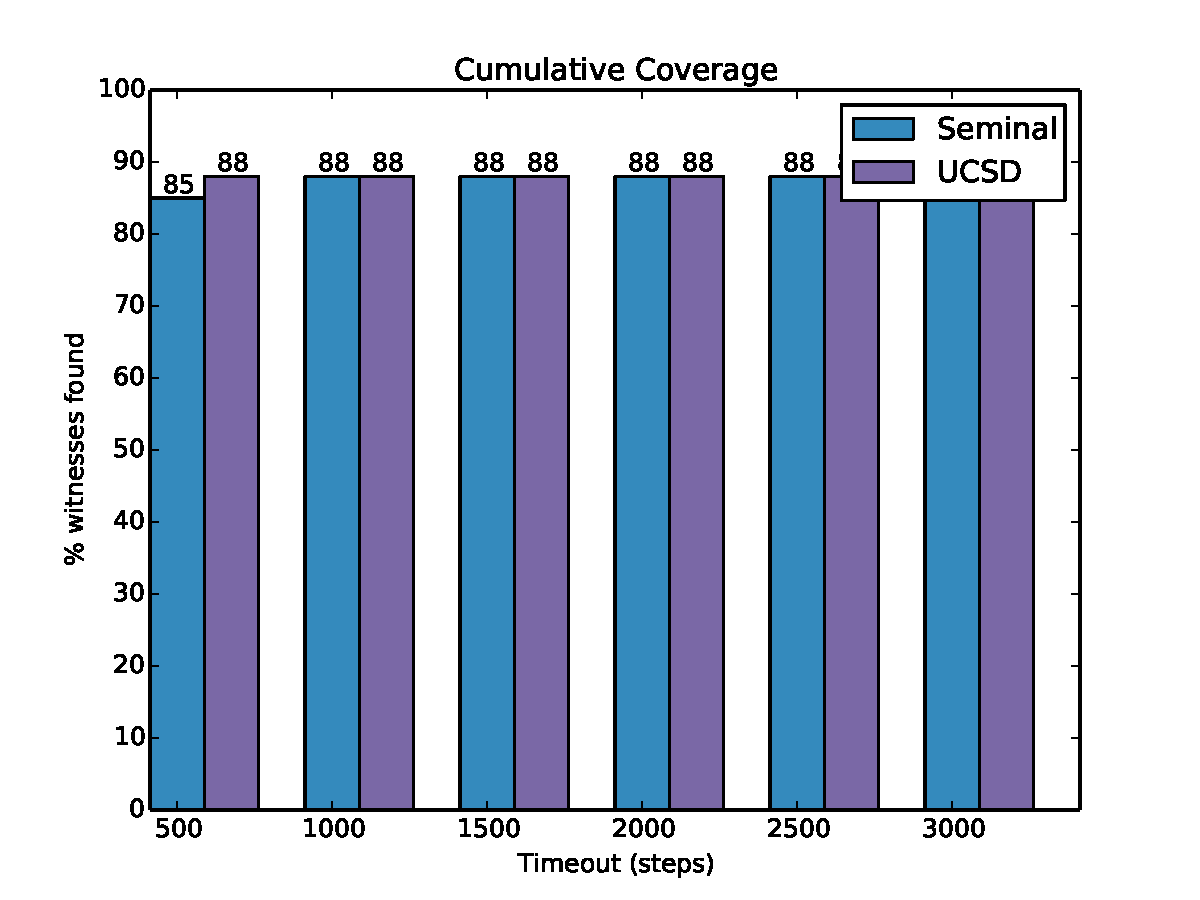
\includegraphics[width=\linewidth]{coverage.pdf}
\end{minipage}
\begin{minipage}{\linewidth}
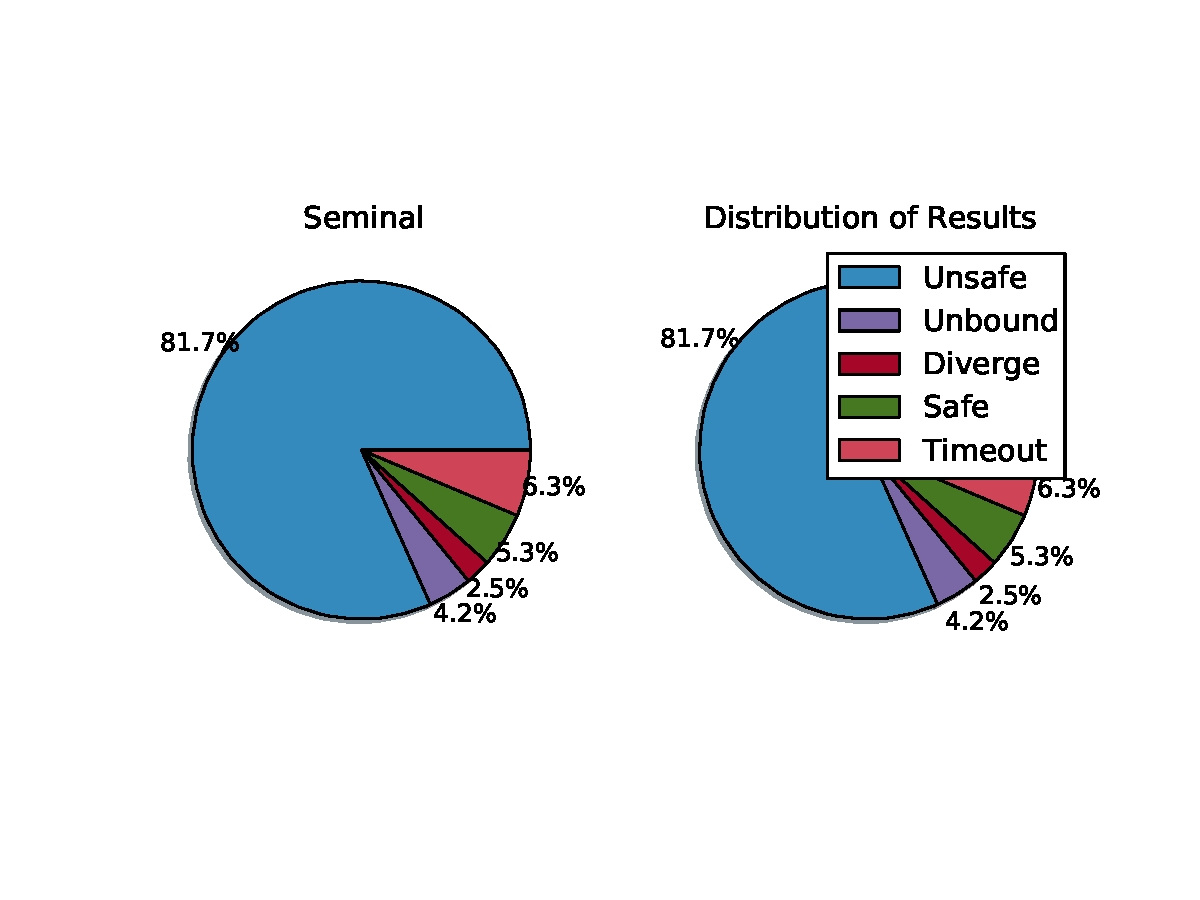
\includegraphics[width=\linewidth]{distrib_seminal.pdf}
\end{minipage}
  % 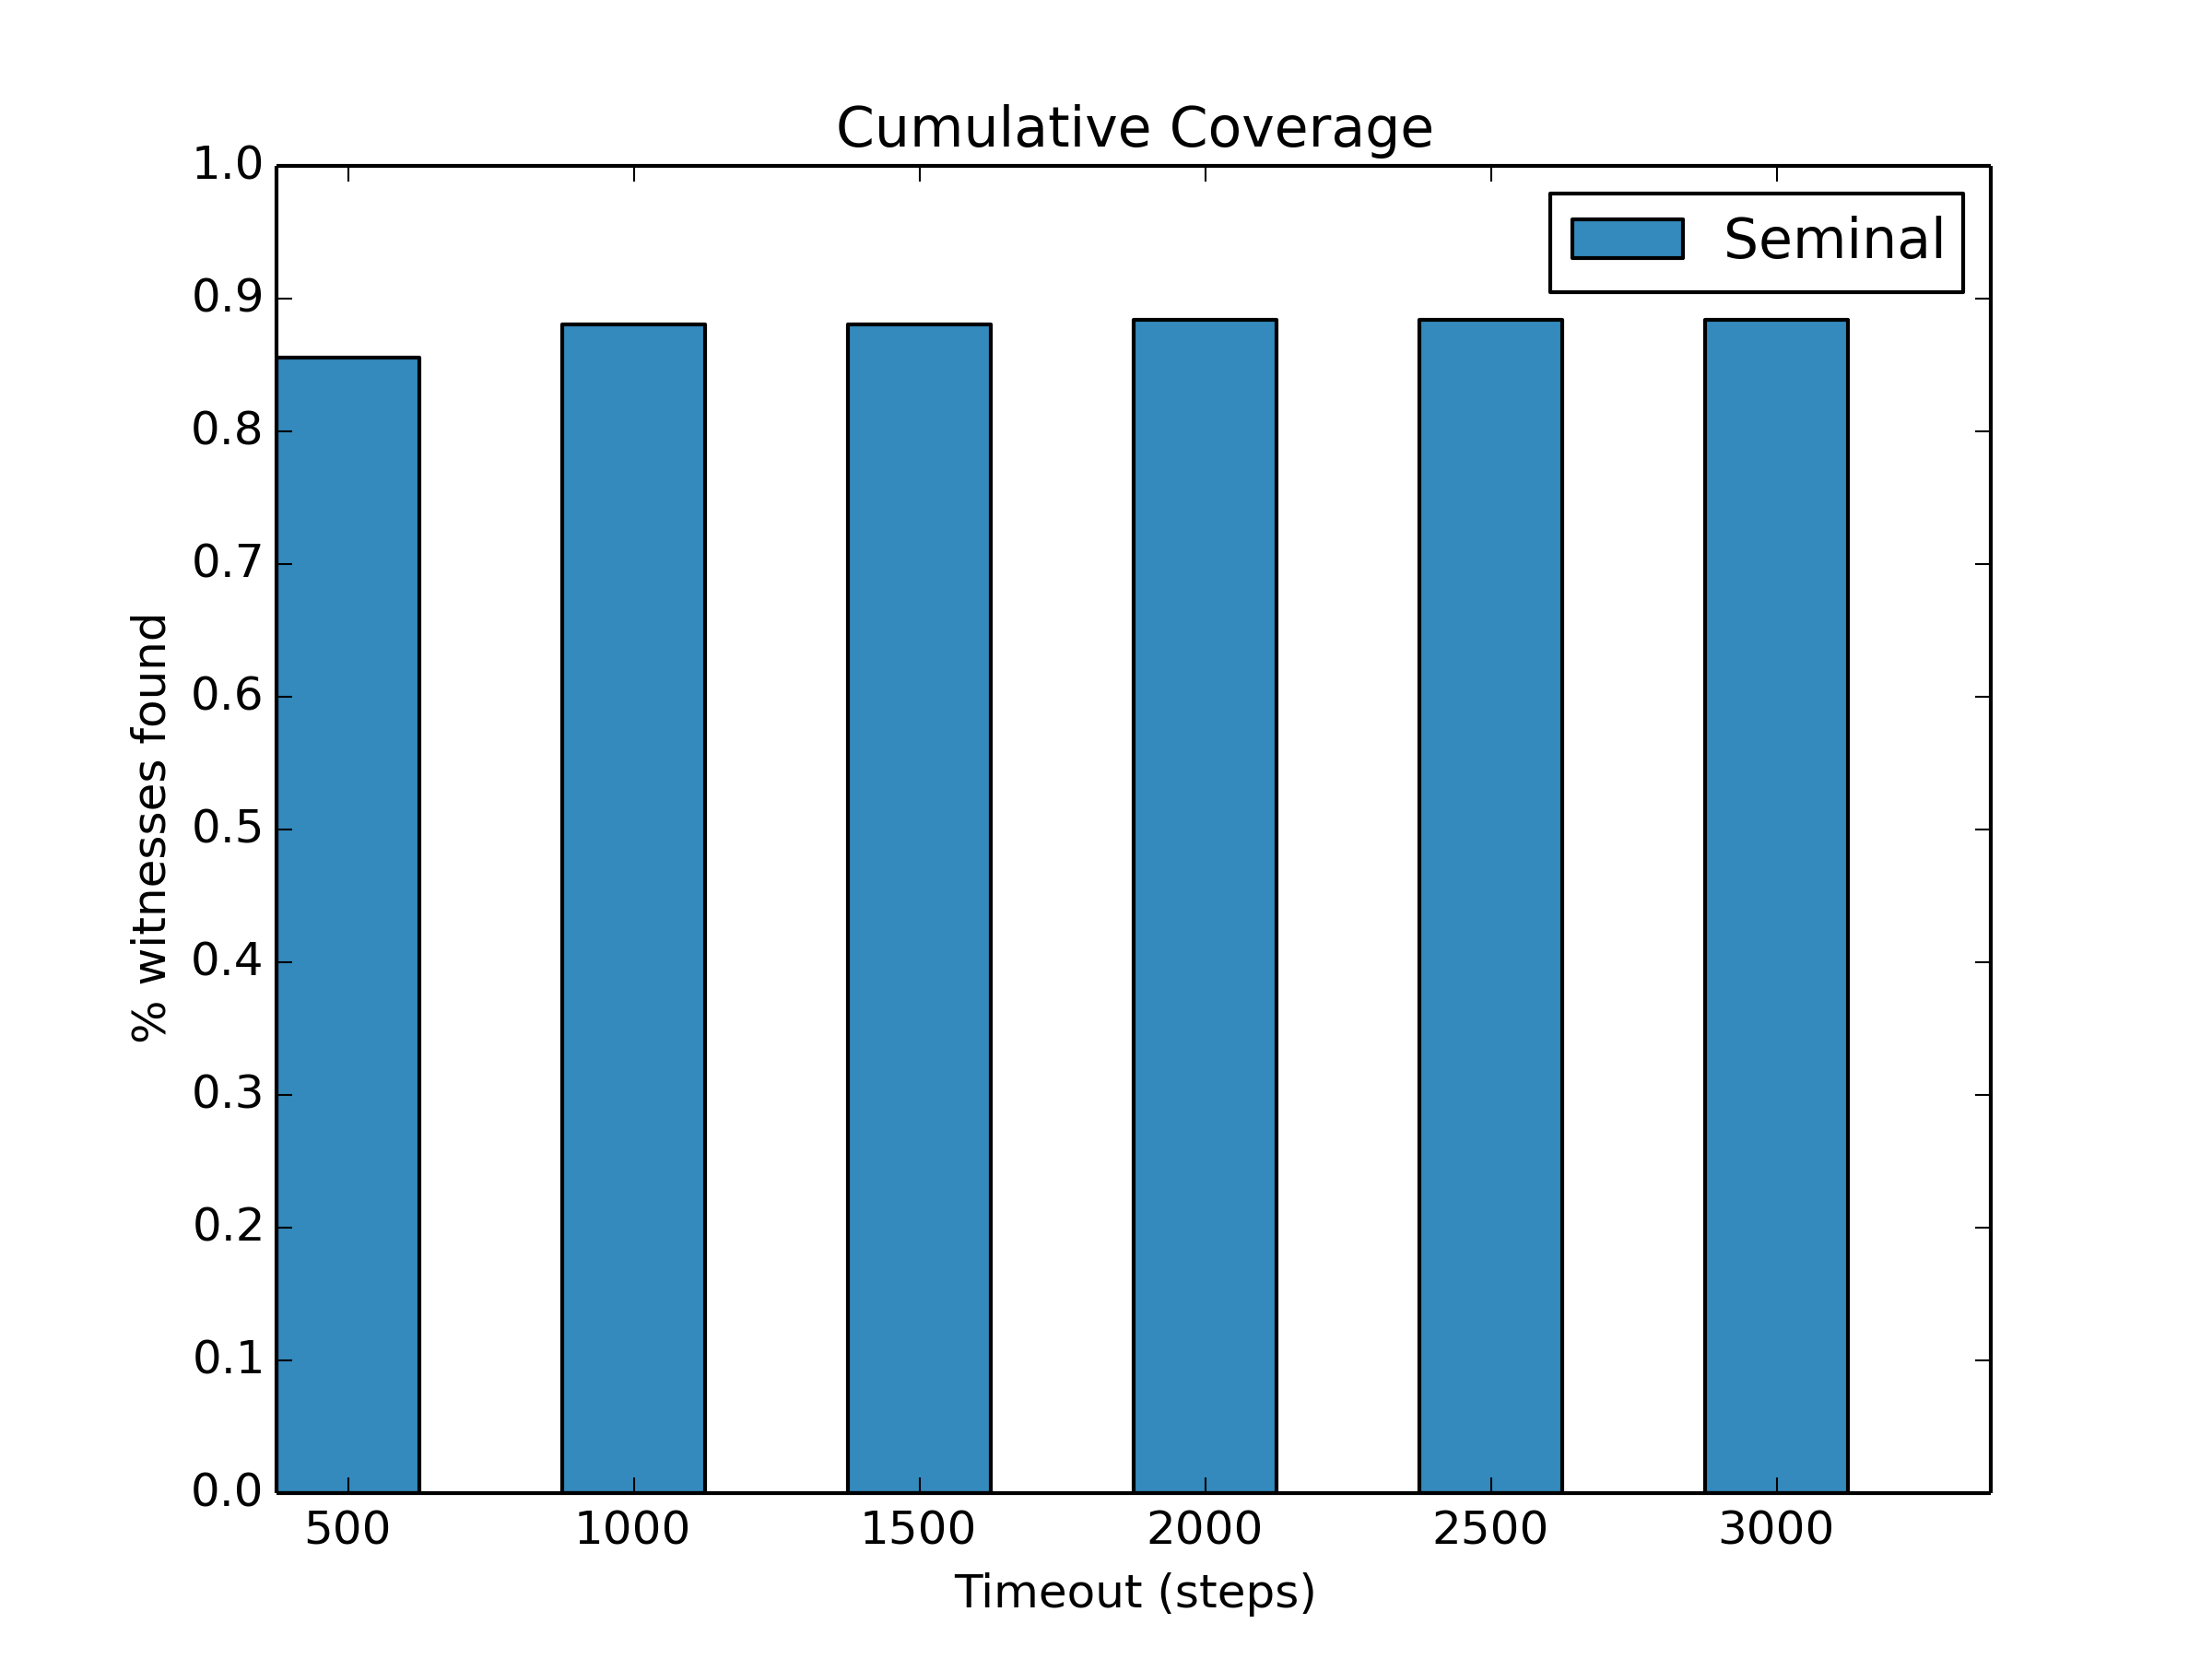
\includegraphics[width=\linewidth]{coverage.png}
  % 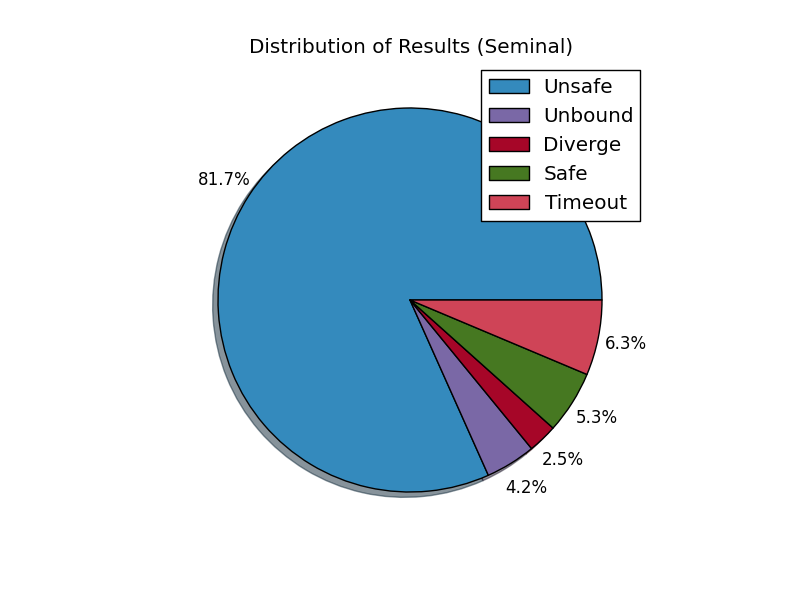
\includegraphics[width=\linewidth]{distrib_seminal.png}

% \begin{tikzpicture} 
% \begin{axis}[
%   title=Cumulative Coverage,
%   ybar interval,
%   xticklabel=
% \pgfmathprintnumber\tick--\pgfmathprintnumber\nexttick
% ]
%     \addplot+[hist={bins=3, cumulative}]
%         table[row sep=\\,y index=0] {
%         data\\
%         1\\ 2\\ 1\\ 5\\ 4\\ 10\\
%         7\\ 10\\ 9\\ 8\\ 9\\ 9\\
%     };
% \end{axis}
% \end{tikzpicture}

% \begin{tikzpicture} \begin{axis}[
%   title=Result Distribution,
% %  ybar interval,
% %  symbolic hist/data coords={S,U,B,O,D,T},
%   hist/symbolic coords={S,U,B,O,D,T},
% %  xticklabel={[\tick--\nexttick[}],
% ]
%     \addplot+[hist={bins=3}]
%         table[row sep=\\,y index=0] {
%         data\\
%         S\\ S\\ U\\
%     };
% \end{axis}
% \end{tikzpicture}

  % Have a table or graph! \ES{graph of cumulative errors per timeout? \ie
  %   monotonically increasing, with a cap of 90\% or so}
\caption{Experimental results}
\label{fig:results-witness}
\end{figure}

\paragraph{Results}
\label{sec:results-witness}
The results of our experiments are summarized in
Figure~\ref{fig:results-witness}.
%
In both datasets our tool was able to find a witness for at least XX\%
of the programs.
%
Interestingly, while the vast majority of witnesses corresponded to a
type-error, as expected, X\% triggered an unbound variable error and X\%
triggered an infinite recursion error.
%
XX programs were deemed safe and XX timed out even at 10,000 steps, \ie
we could not provide any useful feedback for XX\% of the total programs.
%
While a more advanced search procedure, \eg dynamic-symbolic execution,
could likely trigger more of the type errors, our experiments show that
type errors are coarse enough (or that novice programs are \emph{simple}
enough) that these techniques are not necessary.



% \begin{itemize}
% \item benchmarks: our data + seminal data
% \item both cases: \textbf{random} search sufficient to trigger runtime crash in 80\% of programs
% \item how many of the ``safe'' programs are actually safe??
% \end{itemize}


%\section{``Interactive'' Semantics \& Trace Exploration} % 2 pages
\section{Explaining Type Errors With Traces}
\label{sec:interactive}

A trace, on its own, is too detailed to be
a good explanation of the type error. One approach
is to use the witness input to step through the
program with a \emph{debugger} to observe how
the program evolves.
%
This route is problematic for two reasons.
%
First, existing debuggers and interpreters for
typed languages (\eg\ \ocaml) typically require
a type-correct program as input.
%
Second, we wish to have a quicker way to get
to the essence of the error, \eg\ by skipping
over irrelevant sub-computations, and focusing
on the important ones.

Next, we present a novel way to debug executions.
%
First, we develop a notion of a \emph{reduction graphs}
and extend our semantics with a form of \emph{tracing}
so that they incrementally collect the edges
in the graph (\S~\ref{sec:inter-semant}).
%
Next, we express a set of common \emph{interactive debugging}
steps as graph traversals (\S~\ref{sec:traversing-graph}), yielding
an novel interactive debugger that allows the user
to effectively visualize \emph{how} the program goes (wrong.)

% The trace takes the form of a \emph{reduction graph}, where the nodes
% are terms and the edges represent either the single-step
% $\hookrightarrow$ or a ``sub-term'' relation. For example, evaluating
% the expression @1 + 2 + 3@ would produce the graph in
% Figure~\ref{fig:simple-reduction}.
% %
% \begin{figure}[t]
%   \centering
%   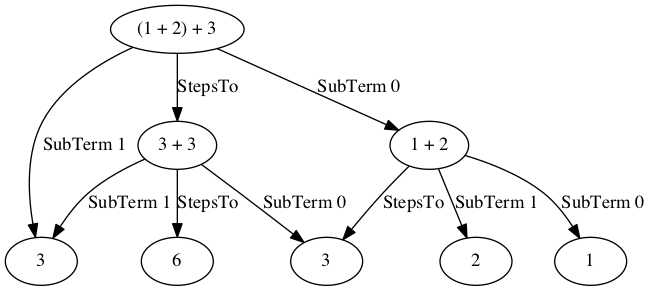
\includegraphics[width=\linewidth]{simple.png}
% \caption{The reduction graph for \texttt{1 + 2 + 3}.}
% \label{fig:simple-reduction}
% \end{figure}
% %
% We choose this graph representation instead of a simple, linear sequence
% of expressions because it will allow us to express a variety of
% traversals, such as ``step into'' and ``step over'' -- commonly found in
% traditional debuggers.



\subsection{Tracing Semantics}
\label{sec:inter-semant}
%
\begin{figure*}[t]
% \relDescription{Trace Syntax}
% $$
% \begin{array}{rrcl}
  % & \tr & ::= & \bullet \spmid \singlestep{e}{e}; \tr \spmid \subterm{e}{e}; \tr
% \end{array}
% $$
% \\
\relDescription{Computing Sub-Terms}
\begin{gather*}
\begin{array}{lcl}
\subtermssym                 & \dcolon & e \to \tr \\
\subterms{\eapp{e_1}{e_2}}   & \defeq & \subterm{\eapp{e_1}{e_2}}{e_1}; \subterm{\eapp{e_1}{e_2}}{e_2} \\
\subterms{\eplus{e_1}{e_2}}   & \defeq & \subterm{\eplus{e_1}{e_2}}{e_1}; \subterm{\eplus{e_1}{e_2}}{e_2} \\
\subterms{\eif{e_1}{e_2}{e_3}}   & \defeq & \subterm{\eif{e_1}{e_2}{e_3}}{e_1}; \\
                                &        & \subterm{\eif{e_1}{e_2}{e_3}}{e_2}; \\
                                &        & \subterm{\eif{e_1}{e_2}{e_3}}{e_3} \\
\subterms{\elet{x}{e_1}{e_2}}   & \defeq & \subterm{\elet{x}{e_1}{e_2}}{e_1}; \\
                                &        & \subterm{\elet{x}{e_1}{e_2}}{e_2} \\
\subterms{\efun{x}{e}}       & \defeq & \subterm{\efun{x}{e}}{e} \\
\subterms{e}                 & \defeq & \bullet
\end{array}
\end{gather*}
\judgementHead{Traced Evaluation}{\stepg{e}{\su}{\tr}{e}{\su}{\tr}}
\begin{gather*}
\inference[\recontext]
  {\stepg{e}{\su}{\tr}{e_1}{\su_1}{\tr_1}}
  {\stepg{C[e]}{\su}{\tr}{C[e_1]}{\su_1}{\singlestep{C[e]}{C[e_1]}; \subterms{C[e_1]}; \tr_1}}
\\ \\
\inference[\reappgood]
  {\pair{\efun{x}{e}}{\su_2} = \force{v_1}{\tfun{\thole{}}{\thole{}}}{\su_1}}
  {\stepg{\eapp{v_1}{v_2}}{\su_1}{\tr}
         {e\sub{x}{v_2}}{\su_1;\su_2}{\singlestep{\eapp{v_1}{v_2}}{e\sub{x}{v_2}}; \subterms{e\sub{x}{v_2}}; \tr}}
\\ \\
\inference[\reappbad]
  {\pair{\stuck}{\su_2} = \force{v_1}{\tfun{\thole{}}{\thole{}}}{\su_1}}
  {\stepg{\eapp{v_1}{v_2}}{\su_1}{\tr}{\stuck}{\su_1;\su_2}{\singlestep{\eapp{v_1}{v_2}}{\stuck}; \tr}}
\end{gather*}
\caption{A selection of the operational semantics from
  Figure~\ref{fig:operational}, extended to collect a full reduction
  graph.}
\label{fig:interactive}
\end{figure*}

\paragraph{Reduction Graphs}
%
A \emph{steps-to} edge is a pair of expressions \singlestep{e_1}{e_2}, which
intuitively indicates that $e_1$ steps, in a single step, to $e_2$.
%
A \emph{sub-term} edge is a pair of expressions \subterm{e_1}{e_2}, which
intuitively indicates that $e_1$ contains $e_2$ as a sub-expression.
%
A \emph{reduction graph} is a set of edges:
$$\tr ::= \bullet \spmid \singlestep{e}{e}; \tr \spmid \subterm{e}{e}; \tr$$

\paragraph{Tracing Semantics}
%
We extend the transition relation (\S~\ref{sec:semantics}) to
collect the set of edges corresponding to the reduction graph.
%
Concretely, we extend the operational semantics to
a relation of the form $\stepg{e}{\vsu}{\tr}{e'}{\vsu'}{\tr'}$
where $\tr'$ collects the edges of the transition.

\paragraph{Collecting Edges}
%
Next, we describe the general recipe for extending a transition
rule to collect edges, and provide a selection of examples
in Figure~\ref{fig:interactive}.
%
The steps-to edges are collected by recording the consequent of
each original rule in the trace. That is, each original judgment
\step{e}{\vsu}{e'}{\vsu'} becomes
\stepg{e}{\vsu}{\tr}{e'}{\vsu'}{\singlestep{e}{e'}; \tr}.
%
The sub-term edges are delegated to a helper function \subtermssym\
which adds edges from an expression to each of its
\emph{immediate} sub-expressions.
%
We collect \subtermssym edges after each transition,
to get the following template for the small-step relation:
\[
\stepg{e}{\vsu}{\tr}{e'}{\vsu'}{\singlestep{e}{e'}; \subterms{e'}; \tr}
\]

% After evaluation the reduction graph can be constructed directly from
% the trace $\tr$ as follows:
% \[
% G(\tr) = \pair{\{e \spmid e \in \tr\}}{\tr}
% \]

% \subsection{Traversing the Reduction Graph}
\subsection{Interactive Debugging}
\label{sec:traversing-graph}

Next, we show how to build a visual interactive debugger
from the traced semantics, by describing the visualization
\emph{state} \ie\ what the user sees at any given moment,
the set of \emph{commands} available to user and what
they do, and finally how we use a command to \emph{update}
the visualization state. In the sequel, for clarity of
exposition, we assume we have a (global) trace:
$\stepg{e_0}{\emptysu}{\bullet}{e_n}{\_}{\tr}$, where
$e_0$ and $e_n$ are the \emph{initial} and \emph{final}
expressions respectively.

\paragraph{Visualization State}
%
A \emph{visualization state} @VState@ is a \emph{directed graph}
whose vertices are expressions and whose edges are such
that each vertex has at most one predecessor and at most one
successor. In other words, the visualization state looks
like a set of linear lists of expressions as shown in Figure~\ref{fig:nanomaly-factorial}.
%
The \emph{initial state} is the graph containing a single
edge linking the initial and final expressions.

\paragraph{Commands}
Our debugger supports the following \emph{commands}, each of which
is parameterized by a single expression (vertex) selected from the
(current) visualization state:
%
\begin{itemize}
%
\item \stepforwardsym, \stepbackwardsym:
      show result of a single step forward or backward respectively,
%
\item \jumpforwardsym:
      show result of taking multiple steps (a \emph{``big''} step)
      upto the first beta-reduction forward or backward respectively,
%
\item \stepintosym:
      show result of stepping into a function call in a sub-term,
      isolating it from the context,

\item \stepoversym:
      show result of skipping over a function call in a sub-term.
\end{itemize}

%\begin{figure}[t]
\centering
% \begin{minipage}{0.49\linewidth}
\begin{mcode}
(*\putBefore*) :: (*\vstate*) -> (*\expr*) -> (*\expr*) -> (*\vstate*)
(*\putAfter*)  :: (*\vstate*) -> (*\expr*) -> (*\expr*) -> (*\vstate*)
(*\putRoot*)   :: (*\vstate*) -> (*\expr*) -> (*\vstate*)
(*\getRoot*)   :: (*\vstate*) -> (*\expr*) -> (*\expr*)
(*\getPath*)      :: (*\tr*) -> (*\expr*) -> [(*\expr*)]

(*\getSubterms*) :: (*\vstate*) -> (*\expr*) -> [((*\expr*),(*\ctx*))]
(*\applyCtx*)    :: (*\vstate*) -> (*\expr*) -> (*\ctx*) -> (*\expr*)

findApp    :: (*\vstate*) -> (*\expr*) -> Maybe ((*\expr*),(*\ctx*))
findValue  :: (*\vstate*) -> (*\expr*) -> (*\expr*)

data (*\cmd*) = (*\stepforwardc*) | (*\stepbackwardc*)
         | (*\jumpforwardc*) | (*\jumpbackwardc*)
         | (*\stepoverc*)    | (*\stepintoc*)
\end{mcode}
% data (*\ctx*)
\caption{Graph manipulation and traversal API.}
\label{fig:graph-api}
\end{figure}
% \end{minipage}
% \begin{minipage}{0.49\linewidth}
\begin{figure}[t]
\begin{mcode}
(*\findExpr*) :: (*\vstate*) -> (*\cmd*) -> (*\expr*) -> Maybe (*\expr*)
(*\findExpr*) v c e = case c of
  (*\stepforwardc*) -> 
    let p = (*\getPath*) v e in (p!!1)
  (*\stepbackwardc*) -> 
    let p = (*\getPath*) v ((*\getRoot*) v e) in last p
  (*\jumpforwardc*) -> case (*\findExpr*) v (*\stepforwardc*) e of
    $\eapp{v_1}{v_2}$ -> Just ($\eapp{v_1}{v_2}$)
    e'   -> (*\findExpr*) v c e'
  (*\jumpbackwardc*) -> case (*\findExpr*) v (*\stepbackwardc*) e of
    $\eapp{v_1}{v_2}$ -> Just ($\eapp{v_1}{v_2}$)
    e'   -> (*\findExpr*) v c e'
  (*\stepintoc*) -> findApp v e
  (*\stepoverc*) -> case findApp v e of
    Nothing       -> Nothing
    Just (e', cx) -> applyCtx v (crunch v e') cx

(*\updState*) :: (*\vstate*) -> (*\cmd*) -> (*\expr*) -> Maybe (*\vstate*)
(*\updState*) v c e = case (*\findExpr*) v c e of
  Nothing -> Nothing
  Just e' -> Just (*\$*) case c of
    (*\stepforwardc*) -> (*\putAfter\ v e e'*)
    (*\stepbackwardc*)    -> (*\putBefore\ v e e'*)
    (*\jumpforwardc*) -> (*\putAfter\ v e e'*)
    (*\jumpbackwardc*)    -> (*\putBefore\ v e e'*)
    (*\stepintoc*)    -> (*\putRoot\ v e' (crunch v e') *)
    (*\stepoverc*)    -> (*\putAfter\ v e e'*)
\end{mcode}
% \end{minipage}
% \[
% \begin{array}{lcl}
% \stepforward{G}{p}{e_i}  &\defeq& \left\{\begin{array}{ll}
%     e_j, & \text{where } \singlestep{e_i}{e_j} \in G
%                          \end{array}\right\} \\ \\
% \stepbackward{G}{p}{e_i}  &\defeq& \left\{\begin{array}{ll}
%     e_j, & \text{where } \singlestep{e_j}{e_i} \in G \text{ and } e_j \in p
%                          \end{array}\right\} \\ \\
% \jumpforward{G}{p}{e_i} &\defeq& \text{let } e_j = \stepforward{G}{p}{e_i} \text{ in }
%                          \left\{\begin{array}{ll}
%                          e_j, & \text{if } e_j = \eapp{v_1}{v_2} \\
%                          \jumpforward{G}{p}{e_{j}}, & \text{otherwise}
%                          \end{array}\right\} \\ \\
% \jumpbackward{G}{p}{e_i} &\defeq& \text{let } e_j = \stepbackward{G}{p}{e_i} \text{ in }
%                          \left\{\begin{array}{ll}
%                          e_j, & \text{if } e_j = \eapp{v_1}{v_2} \\
%                          \jumpbackward{G}{p}{e_{j}}, & \text{otherwise}
%                          \end{array}\right\} \\ \\
% \stepinto{G}{p}{e_i} &\defeq& \left\{\begin{array}{ll}
%                          e\sub{x}{v_2}, & \text{if } e_i = C[\eapp{v_1}{v_2}] \text{ and } \singlestep{\eapp{v_1}{v_2}}{e\sub{x}{v_2}}
%                          \end{array}\right\} \\ \\
% \stepover{G}{p}{e_i} &\defeq& \left\{\begin{array}{ll}
%                          C[v], & \text{if } e_i = C[\eapp{v_1}{v_2}] \text{ and } \multistep{\eapp{v_1}{v_2}}{v}
%                          \end{array}\right\}
% \end{array}
% \]
\caption{Rules for updating the reduction graph given a command and a selected expression. \texttt{updState} returns \texttt{Nothing} if the command was not applicable. % \stepintosym and \stepoversym require a traversal of the
  % sub-term edges to decompose $e_i$ into the target expression
  % \eapp{v_1}{v_2} and the context $C$.  \ES{these rules are quite ugly and waste space..}
}
\label{fig:traversing-graph}
\end{figure}

\begin{figure*}[t]
\[
\begin{array}{lcl}
\stepforward{G}{p}{e_i}  &\defeq& \begin{array}{ll}
    e_j, & \text{where } \singlestep{e_i}{e_j} \in G
                         \end{array}\right\} \\ \\
\stepbackward{G}{p}{e_i}  &\defeq& \left\{\begin{array}{ll}
    e_j, & \text{where } \singlestep{e_j}{e_i} \in G \text{ and } e_j \in p
                         \end{array}\right\} \\ \\
\jumpforward{G}{p}{e_i} &\defeq& \text{let } e_j = \stepforward{G}{p}{e_i} \text{ in }
                         \left\{\begin{array}{ll}
                         e_j, & \text{if } e_j = \eapp{v_1}{v_2} \\
                         \jumpforward{G}{p}{e_{j}}, & \text{otherwise}
                         \end{array}\right\} \\ \\
\jumpbackward{G}{p}{e_i} &\defeq& \text{let } e_j = \stepbackward{G}{p}{e_i} \text{ in }
                         \left\{\begin{array}{ll}
                         e_j, & \text{if } e_j = \eapp{v_1}{v_2} \\
                         \jumpbackward{G}{p}{e_{j}}, & \text{otherwise}
                         \end{array}\right\} \\ \\
\stepinto{G}{p}{e_i} &\defeq& \left\{\begin{array}{ll}
                         e\sub{x}{v_2}, & \text{if } e_i = C[\eapp{v_1}{v_2}] \text{ and } \singlestep{\eapp{v_1}{v_2}}{e\sub{x}{v_2}}
                         \end{array}\right\} \\ \\
\stepover{G}{p}{e_i} &\defeq& \left\{\begin{array}{ll}
                         C[v], & \text{if } e_i = C[\eapp{v_1}{v_2}] \text{ and } \multistep{\eapp{v_1}{v_2}}{v}
                         \end{array}\right\}
\end{array}
\]
\caption{Rules for updating the reduction graph given a command and a selected expression. \texttt{updState} returns \texttt{Nothing} if the command was not applicable. % \stepintosym and \stepoversym require a traversal of the
  % sub-term edges to decompose $e_i$ into the target expression
  % \eapp{v_1}{v_2} and the context $C$.  \ES{these rules are quite ugly and waste space..}
}
\label{fig:traversing-graph}
\end{figure*}


\paragraph{Update}
Figure~\ref{fig:traversing-graph} shows how we update the state
for each command.
%
The procedure @findExpr vs cmd e@ traverses $\tr$
and the current visualization state to compute the new
expression that should be added to the visualization state,
and @updState vs cmd e@ then updates the graph
by inserting the new expression appropriately, using one of
the following functions.
%
@putBefore vs e e'@ \hbox{(resp. @putAfter vs e e'@)}
returns the modified version of @vs@ where @e'@ is the
immediate predecessor of @e@ (resp. the immediate successor of @e@);
%
@putRoot vs e e'@ returns the modified version of @vs@ extended
with a new root vertex @e@ and its successor @e'@.
%
% @getRoot vs e@ returns the vertex (expression) obtained
% by transitively following the predecessors of @e@ until a
% source vertex.

@getNext vs e@ returns the immediate successor of @e@ in $\tr$.
%
@getPrev vs e@ computes the path @p@ between @e@ and its immediate
predecessor in the current visualization, and then returns @e@'s immediate
predecessor along @p@.
%
@getSubterms vs e@ traverses the sub-term edges to decompose an
expression into a list of sub-expressions paired with their context.
%
@applyCtx vs e ctx@ applies @ctx@ to @e@, traversing the sub-term edges
in reverse to find the super-term of @e@.
%
\hbox{@findApp vs e@} builds on top of @getSubterms@ to find the first
application sub-term (if any), \ie the first sub-term that looks like
$\eapp{v_1}{v_2}$.
%
@findVal vs e@ traverses the single-step edges to find the final value
that @e@ reduces to.
%
% Note that the sub-term edges $\searrow$ allow us to decompose an
% expression into a sub-expression and the surrounding context, thus
% enabling the \stepintosym\ and \stepoversym\ traversals.

% \RJ{EXAMPLE of interaction from overview goes here}
\begin{figure}[t]
\centering
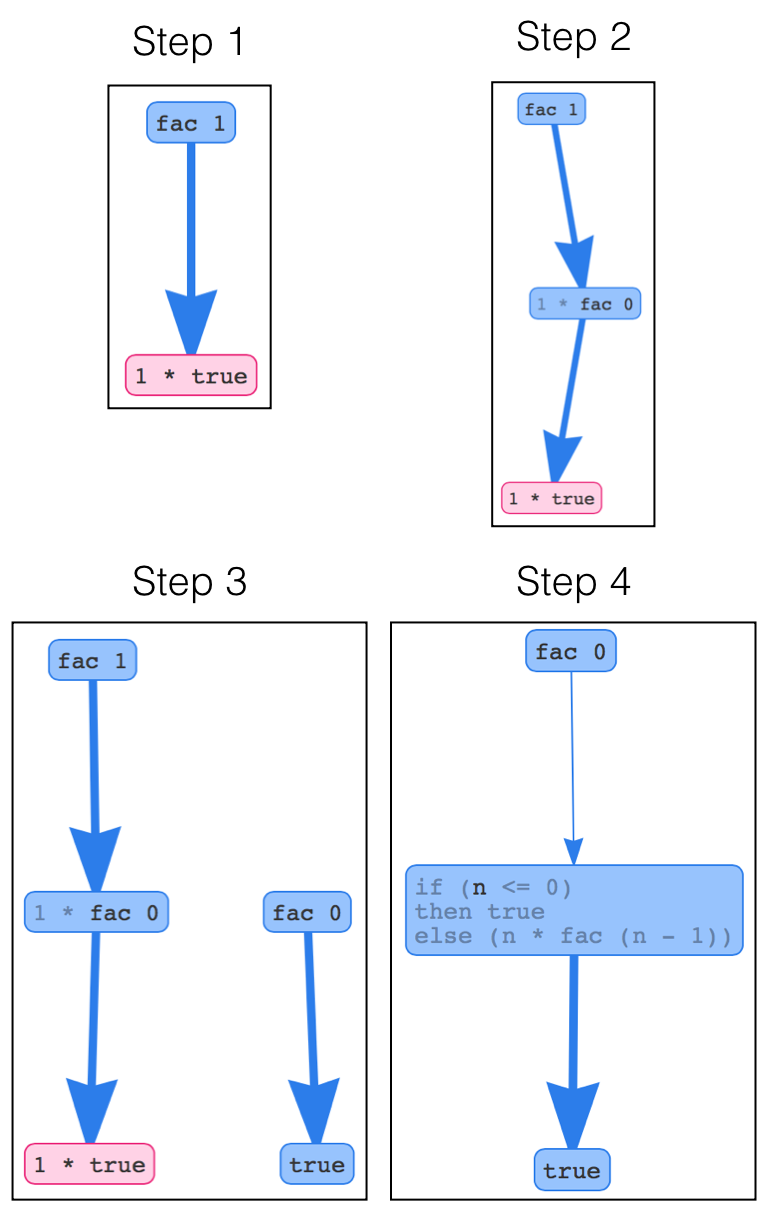
\includegraphics[width=0.8\linewidth]{fac-steps.png}
\caption{A sequence of interactions with the trace of
  \texttt{fac 1}. The stuck term is red, in each node the redex is
  highlighted. Thick arrows denote a multi-step transition, thin arrows
  denote a single-step transition. We start in step 1. In step 2 we jump
  forward from the witness to the next function call. In step 3 we step
  into the recursive \texttt{fac 0} call, which spawns a new ``thread''
  of execution. In step 4 we take a single step forward from
  \texttt{fac 0}.} % (hiding the context for space).}
\label{fig:nanomaly-factorial}
\end{figure}

%
%
%The initial path $p$ is required for the backward-steps as a node may
%have multiple incoming $\leadsto$ edges, \eg
%\singlestep{\eplus{1}{2}}{3} and \singlestep{\eplus{2}{1}}{3}.
%


\section{Evaluation: NanoMaLy}                % 1 page
\section{Related Work}              % 1 pages

\subsection{Type Error Localization}
\label{sec:type-error-local}
\begin{itemize}
\item seminal
\item bayesian (Zhang+Myers)
\item MaxSMT
\item counterfactual (Chen+Erwig)
\end{itemize}
\subsection{Debugging \& Program Understanding}
\label{sec:debugging}



\section{Conclusion}                % 1 page


\end{document}
